\documentclass[11pt]{article}

\usepackage[margin=1in]{geometry}
\usepackage[T1]{fontenc}
\usepackage{lmodern}
\usepackage{microtype}
\usepackage{amsmath, amssymb}
\usepackage{booktabs}
\usepackage{array}
\usepackage{tabularx}
\usepackage{tikz}
\usetikzlibrary{arrows.meta, positioning, shapes.geometric, calc, decorations.pathreplacing, backgrounds}
\usepackage{float}
\usepackage[hidelinks]{hyperref}
\usepackage{caption}
\usepackage{xcolor}
\usepackage{enumitem}
\usepackage[round]{natbib}

\setlength{\parskip}{0.5em}
\setlength{\parindent}{0pt}

\newcommand{\predstart}{\text{pred\_start}}
\newcommand{\predstop}{\text{pred\_stop}}

\title{\textbf{FLAIR Task Schematic} \\[0.3em]
       ICU Daily In-Hospital Mortality at 07:00 Local (Task T1)}
\author{FLAIR Benchmark}
\date{\today}

\begin{document}
\maketitle

\begin{abstract}
\noindent We specify the FLAIR daily ICU in-hospital mortality task:
at every local 07:00 rounds anchor during the first ICU stay, predict
whether the hospitalization will end with the patient dying in hospital,
defined by CLIF \texttt{discharge\_category} $\in
\{\texttt{Expired},\,\texttt{Hospice}\}$. The cohort is all adult ICU
hospitalizations --- \textit{unconditional}: no \texttt{discharge\_category}
filter, every retained stay contributes daily rows, with null and
\texttt{Still Admitted} dispositions kept as label-0. Task T2 shares
the same cohort and grid but with a different (non-complementary)
label.
\end{abstract}

\section{FLAIR operational definition}
\label{sec:def}

\subsection{Anchors and windows}

Let $H_i$ denote a hospitalization with admission time
$t^{\text{adm}}_i$ and discharge or death time $t^{\text{end}}_i =
\min(t^{\text{disch}}_i,\, t^{\text{death}}_i)$. Let
$t^{\text{ICU}_1,\text{start}}_i$ and $t^{\text{ICU}_1,\text{end}}_i$
be the first ICU stay endpoints returned by \verb|compute_icu_timing|
on the CLIF \texttt{ADT} table. All datetimes are naive but
wall-clock-local per \texttt{cfg["timezone"]}; literal hours of the
day are interpreted as local hospital time.

\begin{description}[leftmargin=2em, style=nextline]

\item[Prediction-window start ($\predstart$).]
\[
\predstart_i \;=\; \text{trunc}\!\bigl(t^{\text{ICU}_1,\text{start}}_i,\,
1\text{d}\bigr) + 1\text{d} + 7\text{h}.
\]
The first decision point is local 07:00 on the calendar day \emph{after}
first ICU admission. A patient admitted at 03:00 on Monday gets their
first prediction at 07:00 on Tuesday.

\item[Prediction-window stop ($\predstop$).]
\[
\predstop_i \;=\; \min\!\bigl(t^{\text{ICU}_1,\text{end}}_i,\,
\texttt{coalesce}(t^{\text{death}}_i,\, t^{\text{disch}}_i)\bigr).
\]
Predictions cease at the end of the first ICU stay or the end of the
hospitalization (death if recorded, else discharge), whichever comes
first.

\item[Decision-point grid.]
Daily 24h step:
$D_i = \{\predstart_i + k\!\cdot\!24\text{h} : k\in\mathbb{Z}_{\ge 0},\,
\predstart_i + k\!\cdot\!24\text{h} < \predstop_i\}$.

\item[Label (\texttt{label\_mortality}).]
Let
$\texttt{disp}_i = \texttt{lower}(\texttt{strip}(\texttt{discharge\_category}_i))$.
For $d \in D_i$:
\[
y_i(d) \;=\; \mathbb{1}\!\left[ \texttt{disp}_i \in
\{\,\texttt{"expired"},\, \texttt{"hospice"}\,\} \right].
\]
A null \texttt{disp}$_i$ (i.e., \texttt{discharge\_category} null in
the source) or any non-matching value (Home, SNF, Rehab, LTACH, AMA,
Other, \texttt{Still Admitted}, \ldots) yields $y_i(d) = 0$. The label
is constant across all rows of $H_i$ (the hospitalization's eventual
disposition is a single fact broadcast to every grid point).

\end{description}

\subsection{Cohort (unconditional)}

\begin{itemize}[leftmargin=2em]
  \item Age at admission $\ge 18$ with valid \texttt{admission\_dttm}
        and \texttt{discharge\_dttm}.
  \item $\geq 1$ ICU ADT record (first ICU stay is defined).
  \item First ICU stay long enough to contain at least one 07:00 grid
        point after the admission day (i.e., $\predstart_i <
        \predstop_i$).
\end{itemize}

There is \textbf{no} \texttt{discharge\_category} filter. Stays
discharged Home, SNF, Rehab, LTACH, AMA, Other, with
\texttt{Still Admitted} status, or with null \texttt{discharge\_category}
all remain in the cohort and carry label-0.

\subsection{CLIF tables and categories used}
\label{sec:t1-clif}

Task~T1 reads three CLIF v2.1 tables.

\begin{table}[H]
\centering
\small
\begin{tabular}{@{}llp{7.0cm}@{}}
\toprule
\textbf{CLIF table} & \textbf{Category column} & \textbf{Usage} \\
\midrule
\texttt{hospitalization} & \texttt{discharge\_category} &
\emph{Label-only}: $y=1$ iff lower/strip value $\in$ \{\texttt{Expired},
\texttt{Hospice}\}; null / \texttt{Still Admitted} / any other value
$\Rightarrow$ $y=0$. No cohort filter on this column. \\
\texttt{adt}             & \texttt{location\_category} & Cohort filter:
$\geq 1$ row with value \texttt{"icu"} (case-insensitive). \\
\texttt{patient}         & ---                         & join only; no
category filter. Provides \texttt{death\_dttm} for \predstop. \\
\bottomrule
\end{tabular}
\caption{CLIF surface for Task~T1. Canonical CLIF
\texttt{discharge\_category} values used by the label (case-insensitive
after lower+strip): \texttt{Expired}, \texttt{Hospice}. All other
canonical values (\texttt{Home}, \texttt{Skilled Nursing Facility
(SNF)}, \texttt{Acute Inpatient Rehab Facility}, \texttt{Long Term
Care Hospital (LTACH)}, \texttt{Acute Care Hospital},
\texttt{Group Home}, \texttt{Chemical Dependency}, \texttt{Against
Medical Advice (AMA)}, \texttt{Assisted Living}, \texttt{Still
Admitted}, \texttt{Missing}, \texttt{Other}, \texttt{Psychiatric
Hospital}, \texttt{Shelter}, \texttt{Jail}) plus null map to label-0.}
\end{table}

Columns selected from each table:
\begin{itemize}[leftmargin=2em, itemsep=0pt]
  \item \texttt{hospitalization}: \texttt{hospitalization\_id},
        \texttt{patient\_id}, \texttt{admission\_dttm},
        \texttt{discharge\_dttm}, \texttt{age\_at\_admission},
        \texttt{discharge\_category}.
  \item \texttt{patient}: \texttt{patient\_id},
        \texttt{sex\_category}, \texttt{race\_category},
        \texttt{ethnicity\_category}, \texttt{death\_dttm}.
  \item \texttt{adt}: \texttt{hospitalization\_id},
        \texttt{location\_category}, \texttt{in\_dttm}, \texttt{out\_dttm}.
\end{itemize}

\section{Algorithmic flow}
\label{sec:flow}

\begin{figure}[H]
\centering
% Algorithmic flowchart for FLAIR ICU daily disposition tasks (T1 mortality / T2 LTACH).
% Both tasks share an unconditional cohort and pipeline; only the final label rule differs.

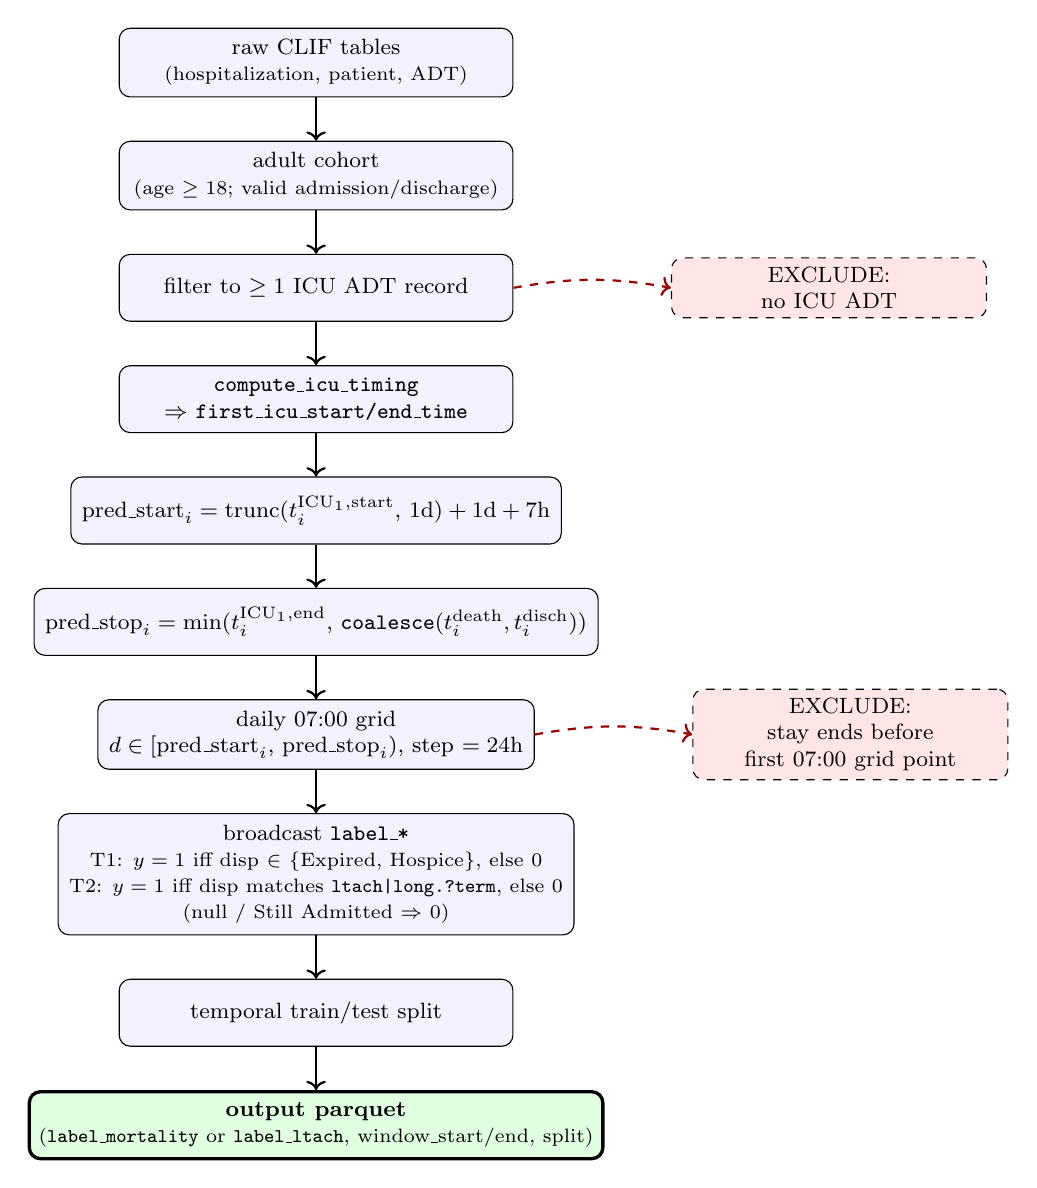
\begin{tikzpicture}[
    node distance=0.55cm and 0.7cm,
    every node/.style={font=\footnotesize, align=center},
    box/.style={draw, rounded corners, fill=blue!5,
                minimum width=5.0cm, minimum height=0.85cm, inner sep=4pt},
    excl/.style={draw, rounded corners, fill=red!10, dashed,
                 minimum width=4.0cm, minimum height=0.7cm},
    outbox/.style={draw, rounded corners, fill=green!12, very thick,
                minimum width=5.0cm, minimum height=0.85cm},
    arrow/.style={->, thick},
    sidearrow/.style={->, thick, red!60!black, dashed},
]
    % main pipeline
    \node[box] (raw)
        {raw CLIF tables\\\scriptsize(hospitalization, patient, ADT)};
    \node[box, below=of raw] (cohort)
        {adult cohort\\\scriptsize(age $\geq 18$; valid admission/discharge)};
    \node[box, below=of cohort] (icu)
        {filter to $\geq 1$ ICU ADT record};
    \node[box, below=of icu] (timing)
        {\texttt{compute\_icu\_timing}\\$\Rightarrow$ \texttt{first\_icu\_start/end\_time}};
    \node[box, below=of timing] (predstart)
        {$\predstart_i = \text{trunc}(t^{\text{ICU}_1,\text{start}}_i,\,1\text{d})
         + 1\text{d} + 7\text{h}$};
    \node[box, below=of predstart] (predstop)
        {$\predstop_i = \min(t^{\text{ICU}_1,\text{end}}_i,\,
         \texttt{coalesce}(t^{\text{death}}_i, t^{\text{disch}}_i))$};
    \node[box, below=of predstop] (grid)
        {daily 07:00 grid\\$d \in [\predstart_i,\, \predstop_i)$, step $= 24$h};
    \node[box, below=of grid] (label)
        {broadcast \texttt{label\_*}\\\scriptsize{T1: $y = 1$ iff disp $\in$
         \{Expired, Hospice\}, else 0}\\\scriptsize{T2: $y = 1$ iff disp matches
         \texttt{ltach|long.?term}, else 0}\\\scriptsize{(null / Still Admitted $\Rightarrow$ 0)}};
    \node[box, below=of label] (split)
        {temporal train/test split};
    \node[outbox, below=of split] (parquet)
        {\textbf{output parquet}\\\scriptsize{(\texttt{label\_mortality} or
         \texttt{label\_ltach}, window\_start/end, split)}};

    % exclusions on the right
    \node[excl, right=2.0cm of icu] (exclNoIcu)
        {EXCLUDE:\\no ICU ADT};
    \node[excl, right=2.0cm of grid] (exclShort)
        {EXCLUDE:\\stay ends before\\first 07:00 grid point};

    % main arrows
    \draw[arrow] (raw) -- (cohort);
    \draw[arrow] (cohort) -- (icu);
    \draw[arrow] (icu) -- (timing);
    \draw[arrow] (timing) -- (predstart);
    \draw[arrow] (predstart) -- (predstop);
    \draw[arrow] (predstop) -- (grid);
    \draw[arrow] (grid) -- (label);
    \draw[arrow] (label) -- (split);
    \draw[arrow] (split) -- (parquet);

    % exclusion arrows
    \draw[sidearrow] (icu.east) to[bend left=10] (exclNoIcu.west);
    \draw[sidearrow] (grid.east) to[bend left=10] (exclShort.west);

\end{tikzpicture}

\caption{Build pipeline shared by Tasks~T1 and T2. The two tasks
consume the same cohort, the same grid, and the same lookback window;
they differ only in the final label predicate. Task~T2 (LTACH) is
detailed in a sibling schematic.}
\label{fig:t1-flow}
\end{figure}

Step-by-step prose:

\begin{enumerate}[leftmargin=2em]
  \item Load CLIF tables: \texttt{hospitalization}, \texttt{patient},
        \texttt{adt}.
  \item Build the adult cohort with valid admission/discharge times.
  \item Restrict to hospitalizations with $\geq 1$ ICU ADT row.
  \item Compute first-ICU-stay window via
        \texttt{compute\_icu\_timing(adt)}.
  \item Compute $\predstart_i$ by truncating
        $t^{\text{ICU}_1,\text{start}}_i$ to date, adding 1 day, then
        adding 7 hours.
  \item Compute $\predstop_i =
        \min(t^{\text{ICU}_1,\text{end}}_i,\,
        \texttt{coalesce}(t^{\text{death}}_i, t^{\text{disch}}_i))$.
  \item Explode the daily 07:00 grid
        $[\predstart_i,\, \predstop_i)$ per hospitalization
        (\verb|pl.datetime_ranges|, $\texttt{interval}=\texttt{"24h"}$,
        \texttt{closed="left"}).
  \item Broadcast the label
        ($\texttt{disp}_i \in \{\texttt{"expired"},
        \texttt{"hospice"}\}$, null-safe via \texttt{fill\_null(False)})
        to every grid row.
  \item Assign \texttt{window\_start} $= d - 24\text{h}$,
        \texttt{window\_end} $= d$ (fixed 24h lookback).
  \item Apply temporal train/test split per
        \texttt{flair\_benchmark.\_split.assign\_split}, keyed on
        \texttt{prediction\_dttm}.
  \item Select \texttt{OUTPUT\_COLS} and persist as parquet.
\end{enumerate}

\section{Design choices and rationale}
\label{sec:rationale}

\paragraph{Why an unconditional cohort.}
Earlier drafts of T1 used a conditional-on-non-survival cohort
(\texttt{discharge\_category} $\in$ \{LTACH, Expired, Hospice\}) to
manufacture a balanced binary task. We dropped that design: it
conflated the cohort filter with the label predicate, made the per-row
positive rate uninterpretable as ``ICU mortality risk,'' and produced
a paired-task framing (T1 $+$ T2 $=$ 1) that misrepresented the
clinical question. The unconditional design is the standard form of
ICU in-hospital mortality prediction \citep{johnson2016mimiciii} and
makes the per-row positive rate a meaningful ICU mortality prevalence.
The task is heavily imbalanced (expected $\sim$10--15\% per-row
positive in MIMIC-CLIF); we report AUPRC alongside AUROC.

\paragraph{Why 07:00 local rounds anchor.}
ICU morning rounds are the canonical decision cadence; predictions
produced before rounds are actionable that day, predictions after
rounds are not. The 07:00 timestamp is a wall-clock-local literal,
relying on \texttt{flair\_benchmark.\_clif.pd\_to\_pl} having stripped
timezone info from \texttt{clifpy} datetimes (which themselves are
typed to \texttt{cfg["timezone"]}). Across CLIF sites this is a stable
choice; sites that prefer 06:00 or 08:00 can re-anchor by adjusting
\texttt{PRED\_HOUR} without changing the rest of the pipeline.

\paragraph{Why daily (not hourly).}
The decision being modeled --- terminal-trajectory commitment --- does
not change hour-to-hour. A daily cadence matches the clinical question
and keeps row counts manageable.

\paragraph{Why Hospice counts as mortality.}
CLIF separates \texttt{Expired} (death in hospital) from
\texttt{Hospice} (alive at discharge to hospice services). FLAIR's T1
bundles them: in routine ICU clinical reasoning, transition-to-hospice
is the operational equivalent of a death-in-hospital trajectory ---
goals-of-care have shifted from cure to comfort, and the prediction
horizon for the morning-rounds decision is identical. Sites that want
the strict CLIF definition (Expired only) can adjust the literal-set
in \texttt{task1\_icu\_daily\_mortality.py}.

\paragraph{Why null / Still Admitted are kept as label-0.}
Dropping these would silently shrink the denominator and bias
prevalence upward. Treating them as negatives matches the standard
in-hospital mortality definition: ``did this patient die during this
encounter? If we don't see a death-coded disposition, assume no.''
Sites with persistent \texttt{Still Admitted} contamination in their
CLIF export should investigate that data-quality gap separately.

\section{Out of scope}

\begin{itemize}[leftmargin=2em]
  \item Multi-class extension to alive-other dispositions (Home, SNF,
        Rehab, AMA) or LTACH as a third class.
  \item Hospital-wide (non-ICU) variant.
  \item Input feature engineering and severity-score baselines
        (e.g., APACHE-III \citep{knaus1991apache3}, SAPS-II).
  \item Survival-time / time-to-event variant.
\end{itemize}

\bibliographystyle{plainnat}
\bibliography{references}

\end{document}
